\documentclass{article}

\usepackage{amsthm}
\usepackage{amsmath}
\usepackage{cite}
\usepackage{listings}
\usepackage{multicol}
\usepackage{url}
\usepackage{graphicx}
\graphicspath{ {./imgs/} }

\setlength{\parindent}{4em}
\setlength{\parskip}{1em}


\begin{document}

\pagenumbering{gobble}

\begin{center}
  \textbf{Project Final Report}

  \textit{Derick Anderson and Harshitha Bhaskar, Blackboard: AndersonBhaskar}
\end{center}

\subsubsection*{The Code}

Code for the project can be found on Derick's GitHub
\footnote{https://github.com/dandersonw/db-final-project}.

\section*{Idea}

The core idea of the project is to develop a journaling tool for managing your
reading. Functionality will include, for example, the ability to track your
progress through books from want-to-read to finished, write reviews of books,
and organize books by author and series. To support said functionality will
require a data model for books, authors, reading lists, etc.

We love to read, but lose track of all the information to do with our
reading. It is great to be able to look forward to the things you want to read,
look back on the things you’ve read, and organize your thoughts about your
reading.

\section*{Technical Specifications}

We used Python 3.7 as our frontend and backend language,
its SQLAlchemy library with the
PyMySQL \footnote{https://github.com/PyMySQL/mysqlclient-python}
connector,
the Tkinter GUI framework,
and the pytest testing framework.
We used the MySQL database with the InnoDB engine.
Note that we will utilize only the core features of SQLAlchemy:
most notably we will not utilize its ORM functionality.

\noindent
We will target Ubuntu 18.10, MacOS 10.14, and MySQL 14.14.

\section*{Installation and Usage}

The project is composed of a Python module for the backend
and a standalone Python file for the frontend.
Installation consists of preparing a Python environment,
installing the backend dependencies,
and then installing and configuring the backend.
The frontend needs no installation.
The project README contains more instructions
\footnote{https://github.com/dandersonw/db-final-project}.
Given that you are using an OS version from the
technical specifications section above,
all packages and libraries should be of the latest version available
from your package manager.

\noindent
With the backend installed and configured you can run the GUI
by running \texttt{make run\_ui} in the root of the project directory.

\section*{UML and EER Diagrams}

Due to the way that \LaTeX \ distributes figures
the diagrams are not located exactly at this point,
but they are contained in the document.
They are unchanged from the progress report
because while the schema has been updated somewhat
(with new triggers, constraints)
the structure of our tables has not changed.

\begin{figure}[h]
  \centering
  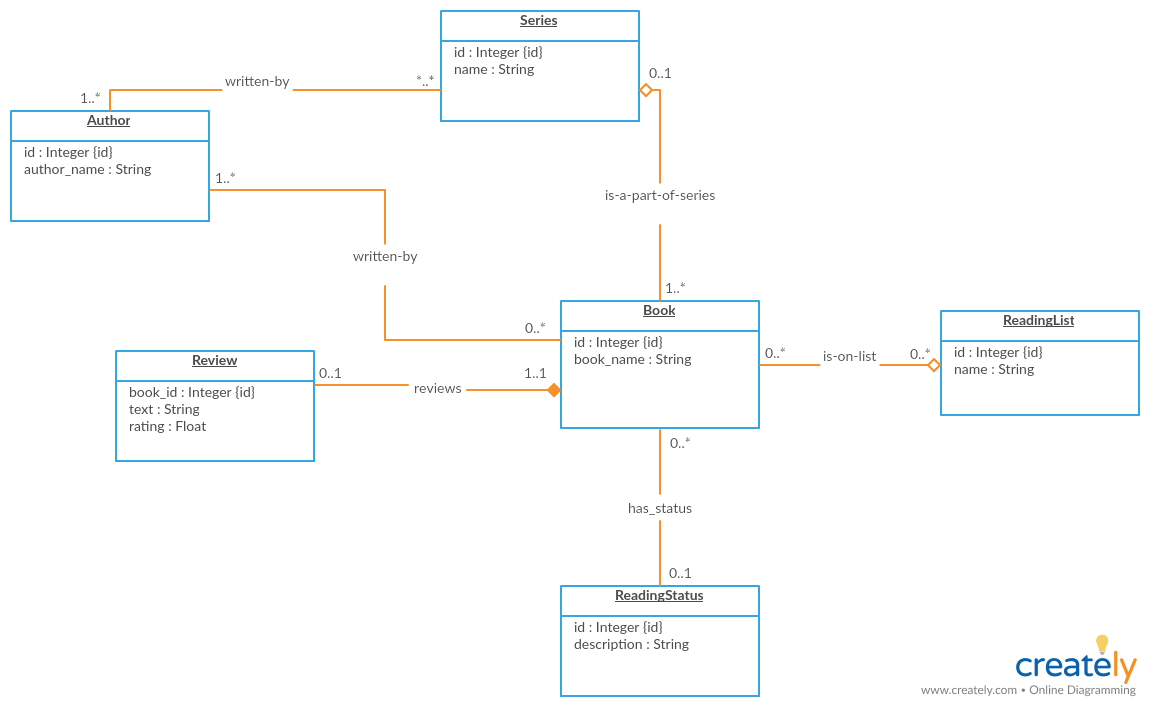
\includegraphics[width=\textwidth]{uml}
  \caption{UML Diagram}
\end{figure}

\begin{figure}[h]
  \centering
  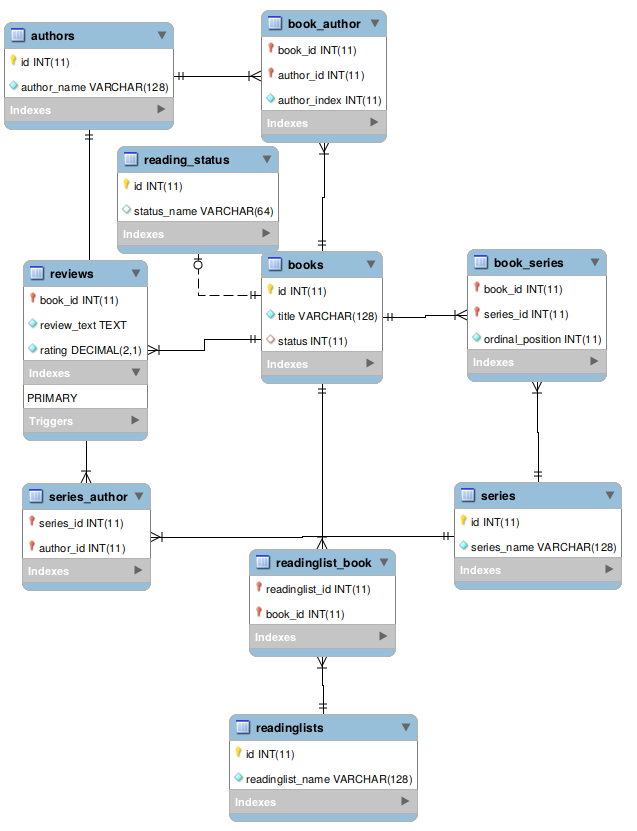
\includegraphics[width=\textwidth]{eer-diagram}
  \caption{EER Diagram}
\end{figure}

\section*{User Flow}

When the user first runs the application, they encounter the main screen of the
application.  This home screen consists of a list of all current books in the
user's reading list, along with the rating, status of completion and series of
the book. All these fields are user defined as this is a personalized, user
specific reading list. Not only does the user have a visual of this, but, they
also have the capability to interact with the list. They have the ability to add
a book, remove a book and edit an existing book. The reading list is not
restricted to books. The user also has the ability to add an author without a
book and add a series without a book or an author.  These extended features give
the user the ability to add an author or series they wish to read in the future
even if they do not have knowledge of the Author's works or the books in a
series.

Going in a little deeper into the home page. The reading list available to the
user is not restricted to the default visible order. The user has the capability
to re-order the list in chronological order (the default order), descending
order of ratings (given that a rating is specified), alphabetic order of the
series the book belongs to (given that a series is specified) and alphabetic
order of the book's author name(given that am author is specified). The user
just needs to click on the appropriately labled button when needed.

\subsubsection*{Adding a Book}

In order to add a book, the user needs to click on the 'Add a Book' button. The
prompts a new window to be opened where the user can enter the book name,
author, series, start date, date of completion, ratings, reviews and reading
status of the book. After entering all information the user deems necessary,
they just needs to click 'Add Book'. This will prompt the window to close and
the book will be seen in the reading list on the homepage. From a backend
perspective, the book will be added to the Books table of the database.

\subsubsection*{Viewing/Editing a Book}

The application gives the user the capability to view in detail and edit any
preexisting book in the database. In order to do this, the user needs to choose
the book from the table and click on the 'View/Edit Book' button on the home
screen. This prompts a new window to be opened with the details of the book that
are available prefilled. The user can now edit the book how they see fit (change
the name, date of start, author, rating, review, etc) and once done editing,
they click "Edit Book" and this will prompt the window to close and the book
will be edited. This edit will be visible in the reading list on the homepage and
from a backend perspective, in the database as well.

\subsubsection*{Adding a Series}

The user can also add a series without having to add a book in that series. To
do this, the user needs to click the 'Add Series' button on the homepage which
prompts a new window to open. Here the user can add the series along with the
author name. Again, the only required field is the name of the series
here. After entering all the information the user wishes to add, they click the
'Add Series' button will prompt the window to close and the series will be added
to the series table. This is visible in the backend database Series table.

\subsubsection*{Adding an Author}

The user can also add an author without having to add a book in that author. To
do this, the user needs to click the 'Add Author' button on the homepage which
prompts a new window to open. Here the user can add the author name. After
entering all the information, the user can click the 'Add Author' button which
will will prompt the window to close and the author will be added to the author
table. This is visible in the backend database Authors table.

On the homepage, the user also has the ability to view all books (with the book
name, series (if available), status of reading and rating, OR they can view just
books and ratings/reviews by clicking the appropriate button between 'Books' and
'Reviews'.

In order to close the application, the user just needs to click the so
appropriately named 'Close' button on the homepage, right above the reading
list.

\section*{Lessons Learned}

\subsubsection*{Technical Expertise Gained}

Derick has some limited experience
working on Python web apps with a database component
(his area of focus is machine learning),
so he found it interesting to without a framework create from scratch
some of the trappings of a real project
(dev/test environments, tests, etc.).

Harshitha had no experience with Python prior to this project. She, however,
does have extensive experience in building full scale applications with MySQL,
but, with Java. This is not the first application she has developed with a MySQL
backend. She found it interesting to see the similarities between the Java Swing
library and Python Tkinter library when it came to UI Development. Not only
this, similarities between connecting MySQL to Java and Python were also
observed and appreciated. One thing, however, she did not get a chance to
research during development was whether it was possible to encode an entire
MySQL Database in Python like possible in Java.

\subsubsection*{Known Issues}

Exceptions are thrown when adding a Book Name-Author pair more than once and
these are not caught. In addition, when attempting to delete a book without
choosing it from the list also throw unhandled exceptions.

Generally speaking,
the frontend is not complete.
The most completely missing functionality is
the ability to interact with reading lists,
although the ability to perform certain operations
on other objects is also missing.
The ability to read, update, or delete authors and series is missing.
Some sorting and organization is missing.

\subsubsection{Time and Group Management}

I (Derick) needed to take a more active role in directing the project.
I had a relatively clear vision for the project,
and I more or less put together the backend necessary,
but failed to ensure that a complementary frontend would be delivered.
That is to say,
as the person with the product vision
I should have communicated that vision more clearly,
and as the (relatively) senior developer
I should have provided more technical support
to the struggling junior developer.
When the frontend was not completed at a late date
I should probably have stepped in more firmly.
(In full honesty,
as this is a school project,
the meaning of ``step in'' is ``do it myself'',
which is the main reason I held off until too late).

\section*{Future Work}

Since we did not complete all of the functionality
that we originally intended to include,
the first item of future work would be finishing our original design.

Functionality not explicitly contemplated by the design
but which would be useful
is the ability to use search to find objects
both in their primary listing screens
and when they need to be input into data fields.
Right now we rely on text input to specify names
which is quite error prone.

\end{document}
%%% Local Variables:
%%% mode: latex
%%% TeX-master: t
%%% End:
